\chapter{Die Schatten von Arkham}
\section{Der Auftrag der Miskatonic University}
\subsection{1.1 -- Ankunft auf dem Universitätsgelände}
\noindent\textbf{Ort:} Miskatonic University, Arkham, Massachusetts\\
\textbf{Zeit:} 5. April 1920, etwa 10 Uhr morgens\\
\textbf{Im Mittelpunkt:} Karim el-Mady (Jörg)


\begin{figure}[htbp]
\centering
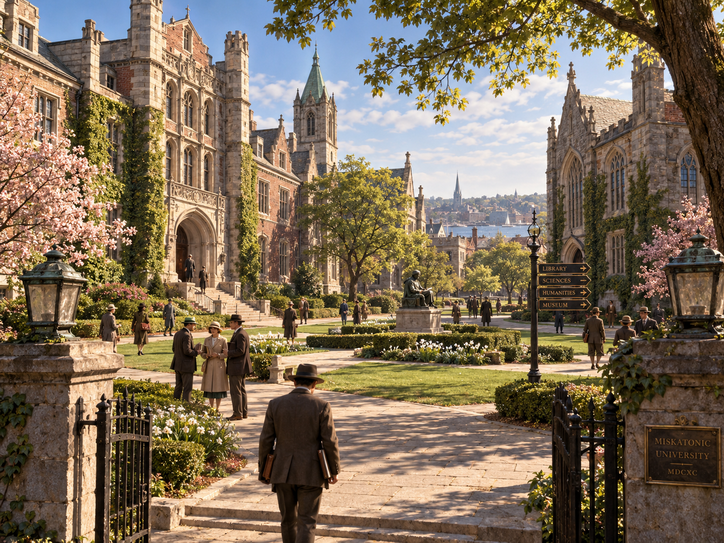
\includegraphics[width=\textwidth]{bilder/miskatonic-campus-im-fruehling.png}
\caption{Die Miskatonic University an einem sonnigen Frühlingsvormittag in Arkham.}
\end{figure}

\begin{vorlesetext}
Es ist ein herrlicher Vormittag in Arkham. Die Sonne steht bereits hoch am nahezu wolkenlosen Himmel und taucht das weitläufige Gelände der altehrwürdigen Miskatonic University in ein warmes, goldenes Licht. Eine leichte Brise bewegt die Blätter der mächtigen Laubbäume, die seit Generationen über die Wege und Grünanlagen des Universitätsgeländes wachen.

Vor Dir erstreckt sich ein beeindruckendes Ensemble ehrwürdiger Bauwerke. Gewaltige Fassaden aus grauem und rötlichem Naturstein erheben sich über sorgfältig angelegten Rasenflächen. Hohe, schmale Fenster mit steinernen Einfassungen durchbrechen die massiven Mauern, während aufwendig gearbeitete Gesimse, Rundbögen und verwitterte Ornamente von der langen Geschichte der Universität zeugen. An manchen Gebäuden rankt sich dichter Efeu bis hinauf zu den oberen Stockwerken. Über den Dächern ragen vereinzelt schlanke Türmchen und reich verzierte Giebel empor.

Trotz ihres beträchtlichen Alters wirken die Gebäude au\ss{}erordentlich gepflegt. Die Fenster glänzen im Sonnenlicht, die steinernen Treppenaufgänge sind sauber gefegt, und selbst die ältesten Mauern strahlen eine gewisse Würde und Beständigkeit aus. Es ist die Art von Ort, an dem man unwillkürlich die Stimme ein wenig senkt, als wolle man die Gelehrsamkeit vergangener Jahrhunderte nicht stören.

Breite, mit hellen Steinplatten gepflasterte Wege durchziehen den Campus und verbinden die zahlreichen Fakultätsgebäude miteinander. Dazwischen liegen kleine, von Blumenrabatten eingefasste Plätze, gepflegte Hecken und schattige Sitzgelegenheiten unter alten Bäumen.

Das Universitätsleben ist bereits in vollem Gange. Junge Männer und Frauen eilen mit Büchern, Ledermappen und zusammengerollten Schriftstücken unter den Armen über die Wege. Einige tragen einfache Kleidung, andere wirken in ihren tadellos sitzenden Anzügen und vornehmen Kleidern beinahe ebenso ehrwürdig wie die Gebäude selbst. Vor einem der gro\ss{}en Eingangsportale stehen drei ältere Herren in dunklen Anzügen beisammen, offenbar in eine angeregte Diskussion vertieft. Einer von ihnen gestikuliert mit einer Pfeife, während die beiden anderen aufmerksam zuhören.

Von einer nahe gelegenen Turmuhr schlägt es zehn.

Du bleibst für einen Augenblick stehen und lässt Deinen Blick über das geschäftige Treiben schweifen. Die Wege verzweigen sich in mehrere Richtungen, führen vorbei an weiteren Gebäuden, durch kleine Grünanlagen und über offene Plätze. An verschiedenen Wegkreuzungen stehen schmiedeeiserne Wegweiser mit sorgfältig beschrifteten Tafeln. Vereinzelt sind an den Eingängen der Gebäude steinerne Schilder und Wappen angebracht.

Irgendwo auf diesem weitläufigen Campus befindet sich das Verwaltungsgebäude, in dem Du um elf Uhr einen Termin beim Präsidenten der Universität hast.

Noch bleibt Dir genügend Zeit, Dich zurechtzufinden.
\end{vorlesetext}

\begin{meisterinfo}
\textbf{Ziel der Szene.} Karim soll eigenständig den Weg zum Verwaltungsgebäude finden. Die Szene gibt ihm etwas Raum, seine Figur kennenzulernen und erste Entscheidungen zu treffen.

\medskip\noindent\textbf{Mögliche Vorgehensweisen:}
\begin{itemize}
\item \textbf{Beschilderung folgen:} Bei näherer Betrachtung der Wegweiser findet Karim Hinweise auf das Verwaltungsgebäude. Keine Fertigkeitsprobe nötig.
\item \textbf{Studierende ansprechen:} Ein vorbeieilender Student kann ihm den Weg erklären -- vielleicht etwas gehetzt, aber höflich.
\item \textbf{Lehrkräfte ansprechen:} Einer der älteren Herren gibt bereitwillig Auskunft und könnte sich nach dem Anlass des Besuchs erkundigen.
\item \textbf{Auf eigene Faust suchen:} Karim kann einen Weg einschlagen; gegebenenfalls gelangt er über einen kleinen Umweg zum richtigen Gebäude.
\end{itemize}

\textbf{Atmosphäre.} Der Einstieg soll ruhig und freundlich wirken. Noch deutet nichts auf das Grauen hin. Die Universität erscheint als Ort der Wissenschaft, Ordnung und Sicherheit.

\textbf{Szenenabschluss.} Frage den Spieler: \emph{\glqq{}Was möchtest Du tun?\grqq{}} 
\end{meisterinfo}

\noindent\textit{Redaktioneller Hinweis: Die Handlung ist derzeit für den 5. April 1920 angesetzt. Der ungewöhnlich warme, fast sommerliche Eindruck wird bewusst als sonniger Frühlingstag beschrieben.}
